\documentclass[tikz,border=8pt]{standalone}
\usepackage[utf8]{inputenc}
\usepackage[T1]{fontenc}
\usepackage{lmodern}
\usepackage{tikz}
\usetikzlibrary{positioning,arrows.meta,fit,backgrounds}

\begin{document}
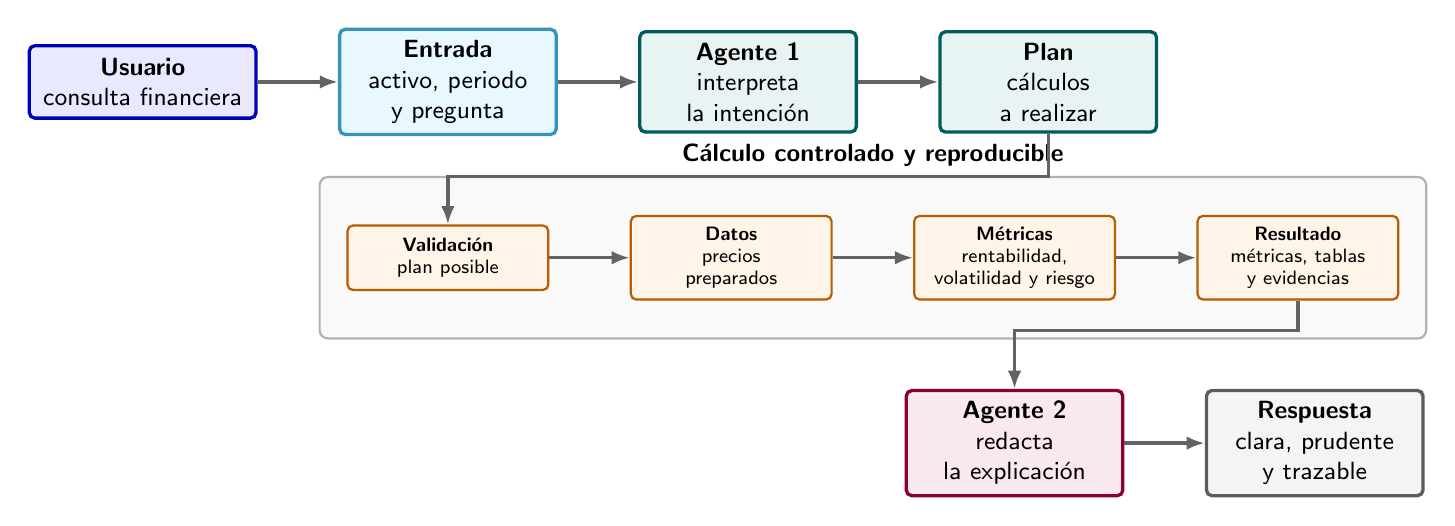
\begin{tikzpicture}[
    font=\sffamily\small,
    node distance=0.72cm and 1.02cm,
    box/.style={
        draw=#1!72!black,
        fill=#1!9,
        rounded corners=2pt,
        very thick,
        align=center,
        minimum width=2.75cm,
        minimum height=0.92cm,
        inner xsep=5pt,
        inner ysep=4pt
    },
    smallbox/.style={
        draw=#1!72!black,
        fill=#1!9,
        rounded corners=2pt,
        thick,
        align=center,
        minimum width=2.55cm,
        minimum height=0.82cm,
        inner xsep=5pt,
        inner ysep=4pt,
        font=\sffamily\scriptsize
    },
    group/.style={
        draw=gray!60,
        fill=gray!5,
        rounded corners=3pt,
        thick,
        inner xsep=0.34cm,
        inner ysep=0.48cm
    },
    arrow/.style={-{Latex[length=2.3mm]}, very thick, draw=gray!78!black}
]

\node[box=blue] (user) {\textbf{Usuario}\\consulta financiera};
\node[box=cyan, right=of user] (input) {\textbf{Entrada}\\activo, periodo\\y pregunta};
\node[box=teal, right=of input] (agent1) {\textbf{Agente 1}\\interpreta\\la intenci\'on};
\node[box=teal, right=of agent1] (plan) {\textbf{Plan}\\c\'alculos\\a realizar};

\node[smallbox=orange, below=1.12cm of input] (validation) {\textbf{Validaci\'on}\\plan posible};
\node[smallbox=orange, right=of validation] (data) {\textbf{Datos}\\precios\\preparados};
\node[smallbox=orange, right=of data] (metrics) {\textbf{M\'etricas}\\rentabilidad,\\volatilidad y riesgo};
\node[smallbox=orange, right=of metrics] (result) {\textbf{Resultado}\\m\'etricas, tablas\\y evidencias};

\begin{scope}[on background layer]
    \node[group, fit=(validation)(data)(metrics)(result), label={[font=\sffamily\small\bfseries]above:C\'alculo controlado y reproducible}] (calcgroup) {};
\end{scope}

\node[box=purple, below=1.12cm of metrics] (agent2) {\textbf{Agente 2}\\redacta\\la explicaci\'on};
\node[box=gray, right=of agent2] (final) {\textbf{Respuesta}\\clara, prudente\\y trazable};

\draw[arrow] (user) -- (input);
\draw[arrow] (input) -- (agent1);
\draw[arrow] (agent1) -- (plan);
\draw[arrow] (plan.south) -- ++(0,-0.54) -| (validation.north);
\draw[arrow] (validation) -- (data);
\draw[arrow] (data) -- (metrics);
\draw[arrow] (metrics) -- (result);
\draw[arrow] (result.south) -- ++(0,-0.38) -| (agent2.north);
\draw[arrow] (agent2) -- (final);

\end{tikzpicture}
\end{document}
